\section{Experimental Results}
\noindent \textbf{Amplification}\\
As mentioned before, the term "DNS reflection and amplification attack" derives from the two key elements involved in the attack methodology. In particular, to achieve amplification the attacker queries the DNS server, which will reply with larger responses than the original requests. In our project, we conducted various tests to explore different amplification factors based on the DNS request used.\\
We have compiled a summary table showcasing the types of DNS requests used, the corresponding response dimensions, and the amplification factors achieved. The table, shown below, provides a comprehensive overview of these metrics.
\begin{table}[H]
    \centering
    \resizebox{\columnwidth}{!}{%
        \begin{tabular}{|l|c|c|c|c|c|}
            \hline
            \textbf{Type} & \textbf{Request} & \textbf{A} & \textbf{MX} & \textbf{NS} & \textbf{ANY} \\
            \hline
            \textbf{Dimension (bytes)} & 74 & 108 & 306 & 330 & 540 \\
            \hline 
            \begin{tabular}[c]{@{}c@{}}\textbf{Amplification} \\ \textbf{Factor}\end{tabular} & - & 1.46 & 4.14 & 4.46 & 7.30 \\
            \hline 
        \end{tabular}%
    }
    \label{tab:dns-amplification}
\end{table}
\noindent \textbf{Effects on the Target}\\
To assess the effects of the DNS reflection attack, various metrics of the targeted system were measured with regards to performance and network aspects. Regarding the network, the target was used as the primary vantage point, and latency was measured using the ping and dig command tools. The measurement process was divided into three sections to analyze the performance differences. Initially, measurements were taken for a minute without any attack. This established a baseline for normal system performance. Subsequently, a two-minute attack was executed, involving the transmission of 10,000 packets per second to the DNS server by multiple attackers. Finally, an additional minute of measurements without any attack was conducted to detect any potential lingering disturbance effects.\\
The latency graph related to DNS queries presented in Figure \ref{fig:Query_MA_ANY1} visually demonstrates the impact of the attack over time. To improve visualization, a moving average of the latency time was applied, revealing a clear trend of increased latency during the attack. This trick becomes particularly helpful considering the inherent instability of latency measurements.
\begin{figure}[H]
    \centering
    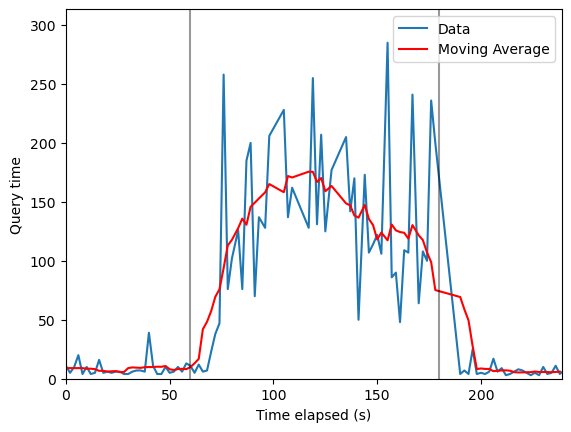
\includegraphics[width=\columnwidth]{Sections/Images/Query_MA_ANY.png}
    \caption{Evolution of the query time over the course of the test with the records of type ANY. The moving average better shows how the latency changes.}
    \label{fig:Query_MA_ANY1}
\end{figure}
\noindent To gain deeper insights into the impact of the DNS reflection attack, it was essential to explore the actual data and analyze the timings of different types of requests. Figure \ref{fig:Boxplots_Query1} showcases the boxplots of query times, illustrating the system under attack with different record types in comparison to the baseline case. \\
\begin{figure}[H]
    \centering
    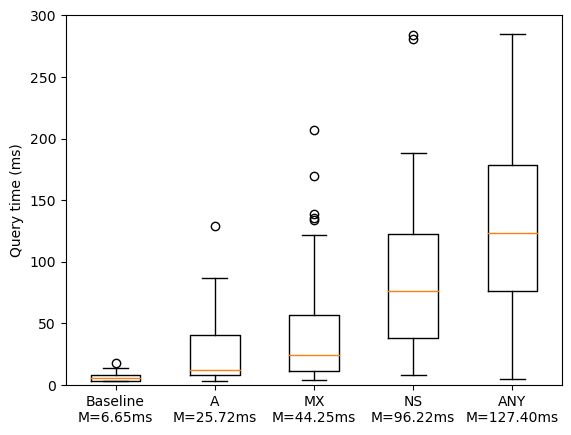
\includegraphics[width=\columnwidth]{Sections/Images/Boxplots_Query.png}
    \caption{Boxplots of the query times with the system under attack with different record types, compared to the baseline case.}
    \label{fig:Boxplots_Query1}
\end{figure}
\noindent By comparing the mean response times during the attack with those observed in the baseline period, we could quantify the magnitude of the latency increase caused by the attack.\\
The results demonstrated that a larger amplification factor corresponds to higher latency. Even in the case of record type A, which typically has a small amplification factor, a noticeable effect on the query time was observed. Remarkably, records of type MX and NS, despite having similar amplification factors (both around 300), exhibited distinct effects on latency. The mean query time for MX records was found to be approximately 44 ms, while NS records had a mean of 96 ms. This discrepancy can be attributed to the resource allocation or in general to the configuration of the DNS server handling the requests.\\
Furthermore, certain cases surpassed the threshold of 100 ms, particularly in the case of the RR ANY record. This indicates that such an attack would have a noticeable impact on the targeted system, for example during web browsing activities. Latencies exceeding this threshold can result in perceptible delays and interruptions, potentially compromising the overall user experience.\\
This analysis provided valuable information on the performance degradation experienced by the targeted system under the influence of the DNS reflection attack.\\
In addition to analyzing the query times using DNS-related tools, we also conducted a similar analysis using the ping command-line tool. The purpose of this analysis was to assess the impact of the DNS reflection attack on overall system latency, beyond just the DNS requests.\\
\begin{figure}[H]
    \centering
    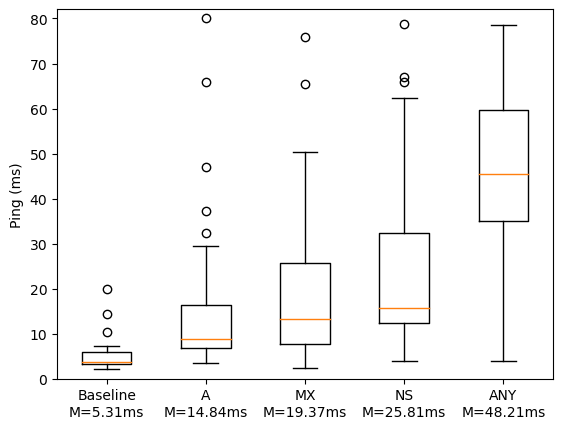
\includegraphics[width=\columnwidth]{Sections/Images/Boxplots_Ping.png}
    \caption{Boxplots of the ping times with the system under attack with different record types, compared to the baseline case.}
    \label{fig:Boxplots_Ping1}
\end{figure}
\noindent As shown in Figure \ref{fig:Boxplots_Ping1} the results obtained from the ping analysis revealed that the latency did not increase significantly during the attack. The highest mean latency observed was approximately 48 ms for the RR of type ANY. \\
This finding suggests that the DNS reflection attack primarily affects the DNS requests themselves, rather than causing widespread disruption to the entire system.\\
During the attacks we also examined the effects of the DNS reflection attack on system resources, specifically RAM and CPU utilization. Our analysis aimed to determine whether the attack had any noticeable impact on these critical resources.\\
Surprisingly, the results revealed that the attack had no significant impact. The resource usage remained within normal ranges, comparable to the baseline measurements taken during the pre-attack phase.\\
\\
\noindent \textbf{Server Performance}\\
The other vantage point of the experiments was the DNS server within the local network. Specifically, the analysis focuses on the CPU and RAM usage to gain insights into the server's behavior during the DNS reflection attacks.
\begin{figure}[H]
    \centering
    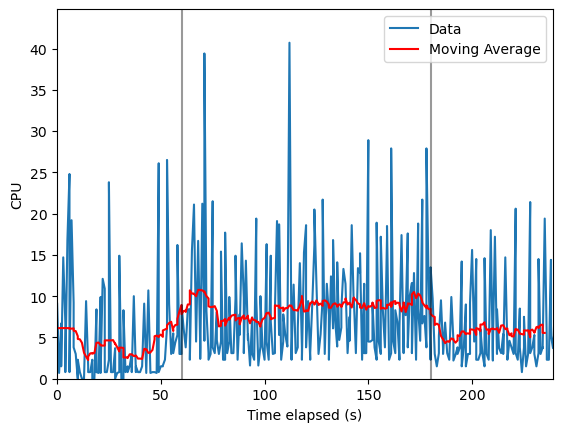
\includegraphics[width=\columnwidth]{Sections/Images/Server_CPU_ANY10.png}
    \caption{Evolution of the DNS server CPU percent used over the course of the attcak with the records of type ANY. The moving average makes the results more clear.}
    \label{fig:Server_CPU1}
\end{figure}
\noindent Figure \ref{fig:Server_CPU1} presents the CPU usage over time, utilizing a moving average to mitigate the volatility of the measurements. Notably, during the attacks, a slight increase in CPU usage is observed, albeit by a marginal 2 to 4\%. This modest change indicates that the CPU's workload experiences a minimal impact during the DNS reflection attacks. While the increased query traffic imposes additional computational demands, the server's CPU manages to handle the heightened workload without significant strain. \\
\begin{figure}[H]
    \centering
    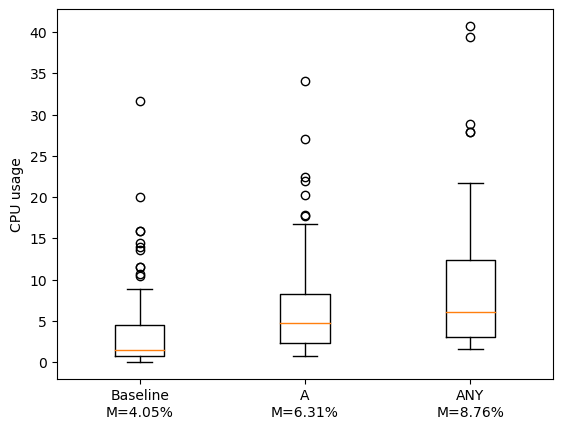
\includegraphics[width=\columnwidth]{Sections/Images/Boxplots_Server.png}
    \caption{Boxplots of the CPU usage with the system under attack with different record types, compared to the baseline case.}
    \label{fig:Boxplots_server}
\end{figure}
\noindent Moving on to the RAM usage, the data reveals a periodic pattern, as shown in Figure \ref{fig:Memory_server}, suggesting the presence of regular garbage collection or memory cleaning processes occurring at intervals. Despite these oscillations, the overall mean value around which the fluctuations occur remains relatively constant. This indicates that the DNS reflection attacks do not significantly affect the server's RAM usage.\\
\begin{figure}[H]
    \centering
    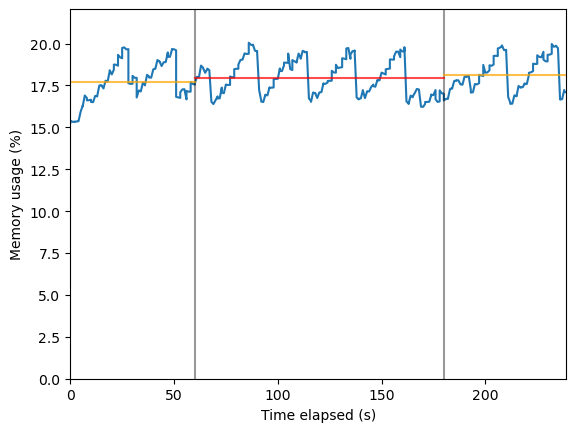
\includegraphics[width=\columnwidth]{Sections/Images/Memory_Server.png}
    \caption{Memory usage of the server during the attack. An oscillating pattern can be observed.}
    \label{fig:Memory_server}
\end{figure}
\noindent The marginal change in CPU usage, coupled with the stable RAM usage, can be attributed to the server's efficient resource management mechanisms. These mechanisms enable the server to effectively handle the increased query load while ensuring minimal impact on CPU and RAM usage.\\
\\
\noindent \textbf{Testing a Big Attack}\\
\noindent In the last test, the focus shifted towards enhancing the potency of the DNS reflection attack. While the previous attacks involved 10,000 packets per second, this more powerful attack reached a traffic 50,000 packets per second, employing the request type "ANY". This intensified attack configuration was aimed to assess the potential for greater disruption and the limits of the network.\\
During this amplified attack, notable changes in DNS query times were observed. The mean query time reached 174 ms, with occasional spikes of 400 ms. These elevated query times would certainly have a substantial impact on the loading speed of web pages. Interestingly, when considering ping latency, the increase was about the same as when using the lower packet rate. The limited increase in latency can be attributed to the server's inability to keep up with the amplified attack: several packets were ignored and were not sent to the spoofed IP, resulting in partial blocking of the reflection. This server behavior lowered the expected proportional increase in latency, as the server struggled to process the influx of requests.\\
\begin{figure}[H]
    \centering
    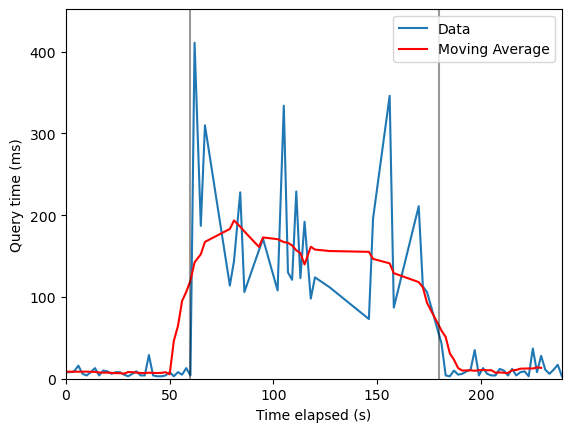
\includegraphics[width=\columnwidth]{Sections/Images/Query_MA_ANY50.png}
    \caption{Query time over the course of the test with a packet rate of 50,000 pps with the requests of type ANY.}
    \label{fig:Query_MA_ANY50}
\end{figure}
\noindent Analyzing the server diagnostics, it was found that the RAM usage remained unaffected by the amplified attack, while on the other hand the strain on the CPU was evident. Unlike the 10,000 packet per second cases, where the CPU usage only experienced a marginal increase, the amplified attack caused the CPU usage to rise significantly. The CPU utilization surged from around 4\% of the baseline to a mean of 24.5\%, with occasional peaks exceeding 30\%. This substantial increase in CPU load indicates the server's struggle to handle the intensified query traffic, resulting in a notable impact on its computational resources.\\
\begin{figure}[H]
    \centering
    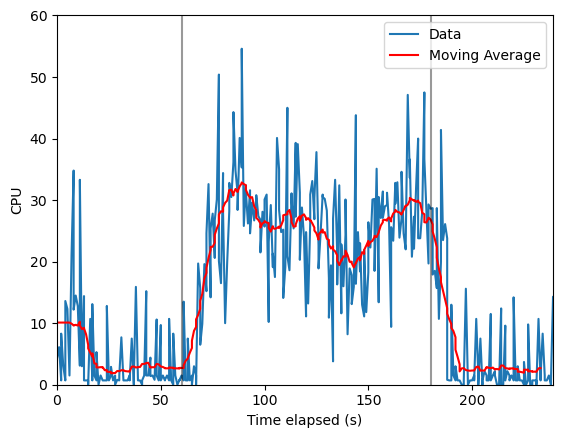
\includegraphics[width=\columnwidth]{Sections/Images/Server_CPU_ANY50.png}
    \caption{CPU usage over the course of the test with a packet rate of 50,000 pps.}
    \label{fig:Server_CPU_ANY50}
\end{figure}
\noindent This final test showed how increasing the attack potency does not always yield the desired effectiveness. The network topology, or in this case the behavior of the server, can exhibit unpredictable characteristics. Despite the significant amplification of the attack, the server's partial blocking and compromised response contributed to unexpected outcomes.\\
\\